\chapter{Governing equations}

Computational fluid-structure interaction (CFSI) combines two separate fields of computational mechanics, computational fluid dynamics (CFD), and computational structure dynamics (CSM). While CFD and CSM traditionally have been considered as two distinct fields of science,  the goal of CFSI is to combine the separate fluid and structure problems ,and their interaction or \textit{coupling} to one another. Therefore, the study CFSI demands understanding of each separate field. This chapter presents the governing equations of the individual fluid and structure problem. Balance laws for each separate problem,  together with auxiliary kinematic, dynamic and material relations will be described briefly.


\section{Continuum Mechanics}
In our effort to understand and describe physical phenomenon in nature, we describe our observations and theories by creating mathematical models. The mathematical models makes scientist and engineers not only able to understand physical phenomena, but also predict them.  All matter is built up by a sequence of atoms, meaning on a microscopic level, an observer will locate discontinuties and space within the material. Evaluating each atom, or \textit{material point}, is not impossible from a mathematical point of view. However, for mathematical moddeling and applications, the evaluation of each material point remains unpractical. In \textit{continuum mechanics}, first formulated by Augustin-Louis Cauchy \cite{Merodio2011}, the microscopic structure of materials are ignored,  assuming the material of interest is \textit{continuously distributed} in space, referred to as a continuum.


In context of this thesis we define a \textit{continuum} as a continuous body $V(t) \subset \mathbb{R}^d \ d \in (1, 2, 3)$ ,  continuously distributed throughout its own extension. The continuum is assumed to be infinitely divisible, meaning one can divide some region of the continuum a indefinitely number of times. A continuum is also assumed to be locally homogeneous, meaning if a continuum is subdivided into infinitesimal regions, they would all have the same properties such as mass density. These two properties forms the baseline for deriving conservation laws and constitute equations, which are essential for formulating mathematical models for the material of interest. However, a continuum remains a mathematical idealization, and may not be a reasonable model for certain applications. In general, continuum mechanics have proven to be applicable provided that $\frac{\delta}{l} << 1$ where $\delta$ is a characteristic length scale of the material micro-structure, and $l$ is a length scale of the problem of interest \cite{Humphrey2002}.

\section{The Lagrangian and Eulerian description of motion}
In continuum mechanics, one makes use if two classical description of motion, the \textit{Lagrangian} and \textit{Eulerian} description. Both concepts are related to an observers view of motion, visually explained by the concepts of \textit{material} and \textit{spatial} points. A material points represents a particle within the material, moving with the material as it move and deform. A spatial point, refers to some reference at which the path of the material points are measured from. 

\begin{figure}[h!]
  \centering
    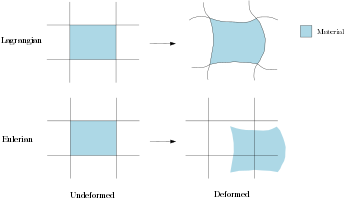
\includegraphics[scale=0.9]{./Fig/lageul.png}
      \caption{Comparison of the Lagrangian and Eulerian description of motion}
\end{figure}


\subsubsection*{Lagrangian}
In the Lagrangian description of motion, the material and spatial points coincide, meaning the reference point of which motion is measured, follows the material as it diverts from its initial position. The initial position of all material points in a continuum extend a region, called the \textit{reference configuration} $\hat{V}$. From now on, all identities in the \textit{reference configuration} will be denoted with the notation "$\wedge$". If a continuum deviates from its reference configuration, a material point $\bat{x}(x, y, z ,t)$ may no longer be at its initial position, but moved to a new position $\mathbf{x}(x, y, z, t)$ at time $t$.  The new positions of all material points extend a new region, called the \textit{current configuration} $V(t)$. 
\newpage

\begin{figure}[h!]
  \centering
    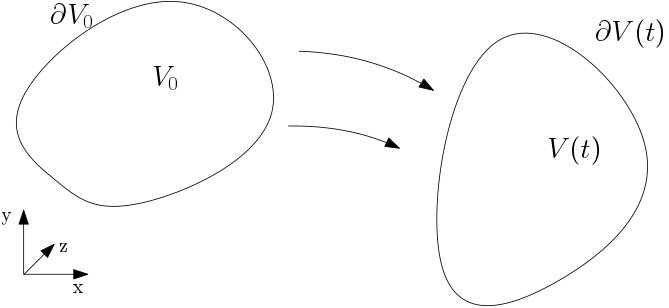
\includegraphics[scale=0.4]{./Fig/unitpotato.png}
      \caption{Unitpotato}
\end{figure}

To measure the displacement of a material point $\mathbf{x} \in V(t)$ for time $t$, from its initial point $\bat{x} \in \hat{V}$, one defines a \textit{deformation vector field} 

\begin{align}
\bat{u}(\ha{x},t) = x(\bat{x},t) - \bat{x} = \ha{T}(\bat{x}, t) 
\end{align}

Mathematically, deformation is a 1:1 mapping  $\ha{T}(\bat{x}, t)$, transforming material points from the   \textit{reference configuration} $\hat{V}$, to the  \textit{current configuration} $V(t)$. Visually, the deformation resembles the shape of continuum for some time $t$. To describe the continuums motion, one defines the \textit{velocity vector field} given by the time derivative of the deformation field,
\begin{align}
\bat{v}(\ha{x},t) = d_t x(\bat{x},t) = d_t \bat{u}(\bat{x},t) = \pder{\ha{T}(\ha{x}, t)}{t} 
\end{align}

The Lagrangian description of motion is the natural choice when tracking particles and surfaces are of main interest. Therefore, it is mainly used within structure mechanics. 

%http://www.brown.edu/Departments/Engineering/Courses/En221/Notes/Kinematics/Kinematics.htm
%Arbitrary Lagrangian-Eulerian methods J. Donea1
\subsubsection*{Eulerian}
 In the Eulerian description, the reference point is kept fixed while the material is deformed.

%The initial shape of the continuum, the \textit{reference configuration}  $V(t = t_0) = \hat{V}$,  is assumed to be stress free.   When the \textit{continuum} undergoes deformation due to applied internal or external forces , the new configuration $V(t)$ for $t \geq t_0$, deviates from its \textit{reference configuration}. The new configuration  $V(t) \neq \hat{V}$, is defined as the \textit{current configuration}. If the continuum undergoes no deformation, the  \textit{reference} and \textit{current} configuration simply coincide. \\ \\




Considering a flow of fluid particles in a river, a \textit{Lagrangian} description of the particles would be tedious as the number of particles entering and leaving the domain quickly rise to a immense number. 
Instead consider defining a view-point $V$ fixed in time, and monitor every fluid particle passing the coordinate $x \in V(t)$ as time elapses. Such a description is defined as the \textit{Eulerian framework.} 
Therefore the Eulerian formulation is natural for describing fluid dynamics. \\
We can describe the particles occupying the \textit{current configuration} $V(t)$ for some time $t \geq t_0$ 
\begin{align*}
x = \ha{x} + \hat{u}(\ha{x}, t)	
\end{align*}
Since our domain is fixed we can define the deformation for a particle 
occupying position $x = x(\ha{x},t)$ as
\begin{align*}
\textbf{u}(x, t) = \hat{u}(\ha{x}, t) = x - \ha{x}	\\
\end{align*}
and its velocity
\begin{align*}
\textbf{v}(x,t) = \partial_t u(x,t) = \partial_t \hat{u}(\ha{x},t) = \hat{v}(\ha{x},t)
\end{align*}

It is important to mention that the we are not interested in which particle is occupying a certain point in our domain, but only its properties. 
%When tracking each particle as it moves, the \textit{material} and \textit{spatial} %points coincide
%As such the \textit{material} and \textit{spatial} points doesn't coincide in the %\textit{Eulerian formulation}

\section{The deformation gradient}
Deformation is a major property of interest when a continuum is influenced by external and internal forces.  The deformation results in relative change of position of material particles, called \textit{strain}. and is the primary property that causes and describe \textit{stress}.

Strain is purely an observation, and it is not dependent on the material of interest. However one expects that a material undergoing strain, will give  forces within a continuum due to neighboring material particles interacting with one another. Therefore one derive material specific models to describe how a certain material will react to a certain amount of strain.
These strain measures are used to define models for \textit{stress}, which is responsible for the deformation in materials \cite{Holzapfel2000}. Stress is defined as the internal forces that particles within a continuous material exert on each other, with dimension force per unit area.  \\

The equations of continuum mechanics can be derived with respect to either a deformed or undeformend configuration. The choice of refering our equations to the current or reference configuration is indifferent from a theoretical point of view. In practice however this choice can have a severe impact on our strategy of solution methods and physical of modelling.   \cite{Wriggers2006}. Regardless of configuration, the \textit{deformation gradient} and \textit{determinant of the deformation gradient} are essential measurement in structure mechanics. 
By \cite{Richter2016}, both configurations are considered.


\subsubsection*{Reference configuration}
\begin{defn}
Let $\hat{u}$ be a differential deformation field in the \textit{reference} configuration, $I$ be the Identity matrix and
the gradient $\hat{\nabla} = (\frac{\partial}{\partial x}, \frac{\partial}{\partial y}, \frac{\partial}{\partial z}) $. Then the \textit{deformation gradient} is given by,
\begin{align}
\bat{F} = I + \hat{\nabla} \bat{u} 
\end{align} 
\textit{expressing the local change of relative position under deformation.}
\end{defn}

\begin{defn}
Let $\hat{u}$ be a differential deformation field in the \textit{reference} configuration, $I$ be the Identity matrix and
the gradient $\hat{\nabla} = (\frac{\partial}{\partial x}, \frac{\partial}{\partial y}, \frac{\partial}{\partial z}) $. Then the \textit{determinant of the deformation gradient} is given by,
\begin{align}
J = det(\bat{F}) = det( I + \hat{\nabla} \bat{u} )
\end{align} 
\textit{expressing the local change of volume the configuration.}
\end{defn}

From the assumption of linear operator \textbf{F}, and no two particles $\bat{x}_a, \bat{x}_b \in \ha{V}$ occupy the same location for some time $V(t)$,  J to be greater than 0 \cite{Wriggers2006}. \\ \\

\subsubsection*{Current configuration}
\begin{defn}
Let $\mathbf{u}$ be a differential deformation field in the \textit{reference} configuration, $I$ be the Identity matrix and
the gradient $\mathbf{\nabla} = (\frac{\partial}{\partial x}, \frac{\partial}{\partial y}, \frac{\partial}{\partial z}) $. Then the \textit{deformation gradient} is given by,
\begin{align}
\mathbf{F} = I - \mathbf{\nabla} \mathbf{u} 
\end{align} 
\textit{expressing the local change of relative position under deformation.}
\end{defn}

\begin{defn}
Let $\mathbf{u}$ be a differential deformation field in the \textit{reference} configuration, $I$ be the Identity matrix and
the gradient $\mathbf{\nabla} = (\frac{\partial}{\partial x}, \frac{\partial}{\partial y}, \frac{\partial}{\partial z}) $. Then the \textit{determinant of the deformation gradient} is given by,
\begin{align}
J = det(\mathbf{F}) = det( I - \mathbf{\nabla} \mathbf{u} )
\end{align} 
\textit{expressing the local change of volume the configuration.}
\end{defn}



\section{The solid problem}

The governing equations for the solid mechanics are given by the balance law,
\begin{equat}
\textit{Solid momentum}
\begin{align}
\rho_s \pder{\bat{v}_s}{t} = \nabla \cdot \bat{S} + \rho_s \mathbf{f}_s
\hspace{4mm} \text{in} \hspace{2mm} \hat{\Omega}_s \\
\pder{\bat{v}_s}{t} = \bat{u_s} \hspace{4mm} \text{in} \hspace{2mm}  \hat{\Omega}_s
\end{align}
\end{equat}
defined in a Lagrangian coordinate system, with respect to an initial reference configuration $\hat{\Omega}_s$. The structure configuration is given by the displacement $\bat{u}_s$, with the relation $\pder{\bat{v}}{t} = \bat{u}_s$ to the solid velocity. The density of the structure is given by $\rho_s$, and $\bat{f}_s$ express any exterior body forces acting. Finally, $\bat{S}$ is the second Piola-Kirchhoff stress tensor, related to the Cauchy-stress tensor by,
 \begin{align*}
 \bat{S}_s = \hat{J} \bat{F}^{-1} \sigma_s \bat{F}^{-T}
 \end{align*}
 
The elasticity of the material is expressed by the \textit{Poisson ratio} $\nu_s$, \textit{Young modulus} E, or Lamè coefficients  $\lambda_s$ and $\mu_s$. Their relation is given by,

\begin{align*}
&E_y = \frac{ \mu_s ( \lambda_s + 2 \mu_s) }{ ( \lambda_s + \mu_s ) } 
\hspace{5mm} \nu_s = \frac{\lambda_s}{2(\lambda_s + \mu_s)} \\
&\lambda_s = \frac{\nu E_y}{(1 + \nu_s)(1 - 2\nu_s)} \hspace{4mm} \mu_s = \frac{E_y}{2(1 + \nu_s)} 
\end{align*}


Material models express the dependency between strain tensors and stress. The validity of material models is often limited by their ability to handle deformation and strain to some extent, before it breaks down or yields nonphysical observations of the material. For small-deformations,  \textit{Hooke's law} assumes a linear relation between strain and stress,

\begin{defn}
Let $\hat{u}$ be a differential deformation field in the \textit{reference} configuration, $I$ be the Identity matrix and the gradient $\hat{\nabla} = (\frac{\partial}{\partial x}, \frac{\partial}{\partial y}, \frac{\partial}{\partial z}) $. \textit{Hooke's law} is then given by,
\begin{align*}
&\sigma_s = \frac{1}{\hat{J}} \bat{F}(\lambda_s(Tr(\epsilon) I + 2 \mu  \epsilon)\bat{F}^{-T} \\
&\bat{S}_s = \lambda_s(Tr(\epsilon) I + 2 \mu \epsilon \\
&\epsilon = \frac{1}{2}(\hat{\nabla} \bat{u} + (\hat{\nabla} \bat{u})^T ) 
\end{align*} 
\end{defn}

Hooke's law is however limited to a small-deformation regime, and is not applicable for larger deformations encountered in this thesis. A valid model for larger deformations is the  hyper-elastic \textit{St. Vernant-Kirchhoff model}(STVK), 
extending Hooke's law into a non-linear regime.

 \begin{defn}
Let $\hat{u}$ be a differential deformation field in the \textit{reference} configuration, $I$ be the Identity matrix and the gradient $\hat{\nabla} = (\frac{\partial}{\partial x}, \frac{\partial}{\partial y}, \frac{\partial}{\partial z}) $. The \textit{St. Vernant-Kirchhoff model} is then given by the relation,
\begin{align*}
&\sigma_s = \frac{1}{\hat{J}} \bat{F}(\lambda_s(Tr(\bat{E}) I + 2 \mu \bat{E})\bat{F}^{-T} \\
&\bat{S}_s = \lambda_s(Tr(\bat{E}) I + 2 \mu \bat{E} \\
&\bat{E} = \frac{1}{2}(\bat{C} - I ) \hspace{4mm} \bat{C} = \bat{F}\bat{F}^{-T}
\end{align*} 
\textit{where $\bat{C}$ is the right Cauchy-Green strain tensor and $\bat{E}$ is the Green Lagrangian strain tensor} \footnote{See appendix A for definition}
\end{defn}
  

Though STVK can handle large deformations, it is not valid for large strain \cite{Razzaq2010}. However since the strain considered in this thesis are small, it will remain our primary choice of strain-stress relation.  STVK describes materials of compressible nature,  but is should be mentioned that for large deformation models describing incompressible materials can be considered. Specially the Incompressible Neo-Hooke (INH) model is considered in several publications (see \cite{Wick2013}, \cite{Richter2010c}), sharing the same hyperelastic properties as the STVK model. While both models are valid for large deformations, the INH is superior compared to STVK in the sense that it holds for large strains aswell \cite{Razzaq2010}. \newpage

As for the fluid problem we define Dirichlet and Neumann boundary conditions on the form

\begin{align*}
\mathbf{v}_s = \mathbf{v}_s^D 
\hspace{4mm} \text{on} \hspace{2mm} \Gamma_s^D \subset \partial \Omega_s  \\
\sigma_s \cdot \mathbf{n} = \mathbf{g}  
\hspace{4mm} \text{on} \hspace{2mm} \Gamma_s^N \subset \partial \Omega_s 
\end{align*}


\section{The Fluid problem}
The fluid is assumed to be express by the in-compressible Navier-Stokes equations,
\begin{equat}
\textit{Navier-Stokes equation}
\begin{align}
&\rho \pder{\mathbf{v}_f}{t} + \rho \mathbf{v}_f \cdot \nabla \mathbf{v}_f =
\nabla \cdot \sigma + \rho \mathbf{f}_f \hspace{4mm} \text{in} \hspace{2mm} \Omega_f \\
&\nabla \cdot \mathbf{v}_f = 0 \hspace{4mm} \text{in} \hspace{2mm} \Omega_f 
\end{align} 
\end{equat}
defined in an Eulerian description of motion. The fluid density as $\rho_f$ and fluid viscosity $\nu_f$  are assumed to be constant in time, and $\mathbf{f}_s$ represents any body force. 
The fluid is assumed Newtonian, where \textit{Cauchy stress sensor} follows Hooke's law
\begin{align*}
\sigma = -p_f I + \mu_f (\nabla \mathbf{v}_f + (\nabla \mathbf{v}_f)^T
\end{align*}

Additional appropriate boundary conditions are supplemented to the equation for a given problem. The first type of of boundary conditions are Dirichlet boundary conditions, 
\begin{align}
\mathbf{v}_f = \mathbf{v}_f^D 
\hspace{4mm} \text{on} \hspace{2mm} \Gamma_f^D \subset \partial \Omega_f 
\end{align}
The second type of boundary condition are Neumann boundary conditions
\begin{align}
\sigma_f \cdot \mathbf{n} = \mathbf{g} 
\hspace{4mm} \text{on} \hspace{2mm} \Gamma_f^N \subset \partial \Omega_f 
\end{align}

